\documentclass[openany]{book}
\usepackage{lmodern}
\usepackage{amssymb,amsmath}
\usepackage{ifxetex,ifluatex}
\usepackage{fixltx2e} % provides \textsubscript
\ifnum 0\ifxetex 1\fi\ifluatex 1\fi=0 % if pdftex
  \usepackage[T1]{fontenc}
  \usepackage[utf8]{inputenc}
\else % if luatex or xelatex
  \ifxetex
    \usepackage{mathspec}
  \else
    \usepackage{fontspec}
  \fi
  \defaultfontfeatures{Ligatures=TeX,Scale=MatchLowercase}
\fi
% use upquote if available, for straight quotes in verbatim environments
\IfFileExists{upquote.sty}{\usepackage{upquote}}{}
% use microtype if available
\IfFileExists{microtype.sty}{%
\usepackage{microtype}
\UseMicrotypeSet[protrusion]{basicmath} % disable protrusion for tt fonts
}{}
\usepackage[margin=1in]{geometry}
\usepackage{hyperref}
\hypersetup{unicode=true,
            pdftitle={Data science for the liberal arts},
            pdfauthor={Kevin Lanning},
            pdfborder={0 0 0},
            breaklinks=true}
\urlstyle{same}  % don't use monospace font for urls
\usepackage{natbib}
\bibliographystyle{apalike}
\usepackage{longtable,booktabs}
\usepackage{graphicx,grffile}
\makeatletter
\def\maxwidth{\ifdim\Gin@nat@width>\linewidth\linewidth\else\Gin@nat@width\fi}
\def\maxheight{\ifdim\Gin@nat@height>\textheight\textheight\else\Gin@nat@height\fi}
\makeatother
% Scale images if necessary, so that they will not overflow the page
% margins by default, and it is still possible to overwrite the defaults
% using explicit options in \includegraphics[width, height, ...]{}
\setkeys{Gin}{width=\maxwidth,height=\maxheight,keepaspectratio}
\usepackage[normalem]{ulem}
% avoid problems with \sout in headers with hyperref:
\pdfstringdefDisableCommands{\renewcommand{\sout}{}}
\IfFileExists{parskip.sty}{%
\usepackage{parskip}
}{% else
\setlength{\parindent}{0pt}
\setlength{\parskip}{6pt plus 2pt minus 1pt}
}
\setlength{\emergencystretch}{3em}  % prevent overfull lines
\providecommand{\tightlist}{%
  \setlength{\itemsep}{0pt}\setlength{\parskip}{0pt}}
\setcounter{secnumdepth}{5}
% Redefines (sub)paragraphs to behave more like sections
\ifx\paragraph\undefined\else
\let\oldparagraph\paragraph
\renewcommand{\paragraph}[1]{\oldparagraph{#1}\mbox{}}
\fi
\ifx\subparagraph\undefined\else
\let\oldsubparagraph\subparagraph
\renewcommand{\subparagraph}[1]{\oldsubparagraph{#1}\mbox{}}
\fi

%%% Use protect on footnotes to avoid problems with footnotes in titles
\let\rmarkdownfootnote\footnote%
\def\footnote{\protect\rmarkdownfootnote}

%%% Change title format to be more compact
\usepackage{titling}

% Create subtitle command for use in maketitle
\newcommand{\subtitle}[1]{
  \posttitle{
    \begin{center}\large#1\end{center}
    }
}

\setlength{\droptitle}{-2em}

  \title{Data science for the liberal arts}
    \pretitle{\vspace{\droptitle}\centering\huge}
  \posttitle{\par}
    \author{Kevin Lanning}
    \preauthor{\centering\large\emph}
  \postauthor{\par}
      \predate{\centering\large\emph}
  \postdate{\par}
    \date{2019-01-05}

\usepackage{booktabs}

\begin{document}
\maketitle

{
\setcounter{tocdepth}{1}
\tableofcontents
}
\hypertarget{section}{%
\chapter*{}\label{section}}
\addcontentsline{toc}{chapter}{}

\hypertarget{an-invitation}{%
\chapter*{an invitation}\label{an-invitation}}
\addcontentsline{toc}{chapter}{an invitation}

This work-in-progress includes my notes for \href{https://kevinlanning.github.io/DataSciSpring2019/}{\emph{\emph{Introduction to Data Science}}} at the Wilkes Honors College of Florida Atlantic University.

Data science is still a new field of study, and there are multiple approaches to teaching it and to its place in the college curriculum. This course is like those at the universities of \href{https://idc9.github.io/stor390/}{North Carolina}, \href{https://github.com/STAT545-UBC/STAT545-UBC.github.io}{British Columbia}, \href{https://www2.stat.duke.edu/courses/Fall15/sta112.01/}{Duke}, \href{http://www.hcbravo.org/IntroDataSci/calendar/}{Maryland}, \href{http://pages.stat.wisc.edu/~yandell/R_for_data_sciences/syllabus.html}{Wisconsin}, \href{https://github.com/dcl-2017-04/curriculum}{Stanford}, \href{https://byuistats.github.io/M335/syllabus.html}{BYU}, \href{http://datasciencelabs.github.io/}{Harvard}, \href{https://github.com/MUSA-620-Spring-2017/Course-Materials}{Pennsylvania}, and \href{https://github.com/FAUDataScience/stat259}{UC Berkeley} (and will likely draw from all of these) in that it is closer to Statistics than to Computer Science.

But if our approach is closer to statistics than to programming, it is particularly close to statistics in its most applied and pragmatic form. The choice of statistical methods should follow from the data and problem at hand - or, as \citet{loevinger1957objective} once put it, statistics should be the handmaiden of real-world concerns rather than technology.

This pragmatic focus is not unique. Courses with similar goals (which we may again draw from) include those at \href{https://github.com/UC-MACSS/persp-analysis}{Chicago}, \href{https://github.com/jacobeisenstein/gt-css-class}{Georgia Tech}, \href{https://github.com/raviolli77/dataScience-UCSBProjectGroup-Syllabus}{UC Santa Barbara}, \href{http://www.princeton.edu/~mjs3/soc596_f2016/}{Princeton}, \href{https://github.com/rochelleterman/PS239T}{UC Berkeley}, at \href{https://github.com/HertieDataScience/SyllabusAndLectures}{Berlin's Hertie School of Governance}, and in \href{https://github.com/tommeagher/data1-fall2015}{Columbia's School of Journalism}.

\hypertarget{what-will-be-in-the-class}{%
\section*{what will be in the class?}\label{what-will-be-in-the-class}}
\addcontentsline{toc}{section}{what will be in the class?}

\textbf{R}

In my 2017 survey of introductory data science courses, I saw a pretty even split between those which begin with Python and those which begin with the statistical programming language R. This difference corresponds, loosely, to the split noted above: Computer science based approaches to data science are frequently grounded in Python, while stats based approaches are generally grounded in R. Our course, like those for most of the syllabi and courses linked above, will be based in R.

\textbf{Reproducible science}

The course will provide an introduction to some of the methods and tools of reproducible science. We will consider the replication crisis in the natural and social sciences, and then consider three distinct approaches which serve as partial solutions to the crisis. The first of these is training in a notebook-based approach to writing analyses, reports and projects (using R markdown). The second is using public repositories (such as the \href{https://osf.io/}{Open Science Framework} and \href{https://github.com/}{GitHub}) to provide snapshots of projects over time. Finally, the third is to consider the place of significance testing in the age of Big Data, and to provide training in the use of descriptive, exploratory techniques of data analysis.

\textbf{Good visualizations}

Part of Type C data science is communication, and this includes not just writing up results, but also designing data displays that incisively convey the key ideas or features in a flood of data. We'll examine and develop data visualizations such as plots, networks and text clouds. More advanced topics may include maps, interactive displays, and animations.

\textbf{\sout{All} \emph{Some of} the data}

It's been \href{https://www.udemy.com/datascience/learn/v4/t/lecture/3473822?start=379}{argued} that in the last dozen years, humans have produced more than 60 times as much information as existed in the entire previous history of humankind. (It sounds like hyperbole, but even if it's off by an order of magnitude it's still amazing). There are plenty of data sources for us to examine, and we'll consider existing datasets from disciplines ranging from literature to economics to public health, with sizes ranging from a few dozen to millions of data points. We will also clean and create new datasets.

\textbf{\sout{All} \emph{Some of} the tools}

In addition to R, we'll use a range of other tools: We'll communicate on the Slack platform. We'll write using markdown editors such as \href{https://typora.io/}{Typora}. We'll certainly use spreadsheets such as Excel or Google Sheets. We \emph{may} use additional tools for visualizing data such as Gephi and Tableau. In any event, \textbf{there will be computing throughout the course.} You will be expected to bring a laptop every day. (Please let Dr.~Lanning know ASAP if you don't have access to this).

\textbf{The place of data science in the WHC (and FAU) curriculum}

At this writing, there is enthusiasm across units of FAU and its affiliated institutes, including Max Planck and FAU's Colleges of Science and Engineering as well as the WHC, for integrating data science into our curriculum. Within the WHC, a data science minor and a multi-track concentration are under development. Until these proposals have been formally approved, students interested in concentrating in Data Science are encouraged to pursue an individual concentration (see Dr.~Lanning for details).

In addition, there are several integrated `4 + 1' pathways which will lead to a master's degree in the College of Engineering. These programs are also in progress; again, see Dr.~Lanning for additional details.

\hypertarget{should-you-enroll}{%
\section*{should you enroll?}\label{should-you-enroll}}
\addcontentsline{toc}{section}{should you enroll?}

It's my intention that this course should serve every Wilkes Honors College student, regardless of concentration. The WHC was built and funded by the state of Florida to train tomorrow's leaders. That's you. The skills and insights that you will gain in this course will help you in graduate and professional schools, will help you in your careers, and will help you in your goal of making a better world. And it will help you train the next generation of data scientists, too.

\textbf{How do I sign up?}

If you are interested in taking the class, complete the Google form \href{https://goo.gl/forms/kXGAOTShcOLPwjPH2}{here}. Note that enrollment in the class and lab will be limited to 30.

\hypertarget{part-introduction}{%
\part{Introduction}\label{part-introduction}}

\hypertarget{data-science-for-the-liberal-arts}{%
\chapter{data science for the liberal arts}\label{data-science-for-the-liberal-arts}}

Hochster, in \citet{hicks2017guide}, describes two broad types of data scientists: Type A (Analysis) data scientists, whose skills are like those of an applied \textbf{statistician}, and Type B (Building) data scientists, whose skills lie in problem solving or coding, using the skills of the \textbf{computer scientist}. This view arguably omits a critical component of the field, as data science is driven not just by statistics and computer science, but also by ``domain expertise:''

\begin{figure}
\centering
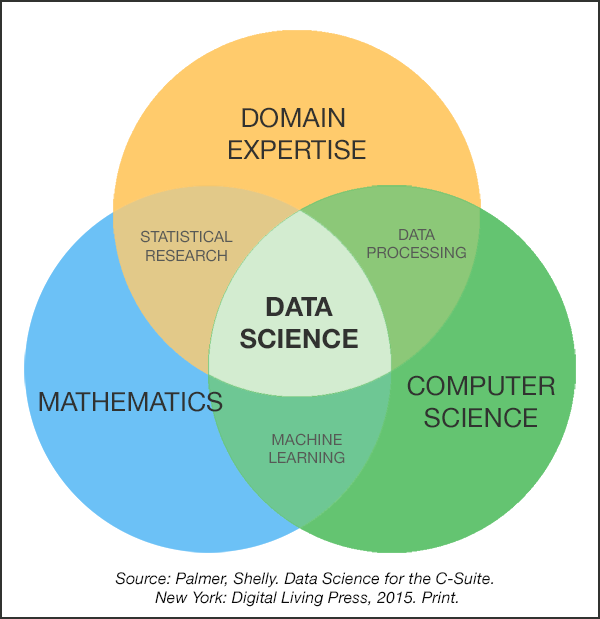
\includegraphics{dataVenn.png}
\caption{\emph{Fig 1.1 - The iconic data science Venn diagram}}
\end{figure}

\hypertarget{type-c-data-science-data-science-for-the-liberal-arts}{%
\section{type C data science = data science for the liberal arts}\label{type-c-data-science-data-science-for-the-liberal-arts}}

The iconic \href{https://www.google.com/search?q=venn+diagram+model+of+data+science\&newwindow=1\&safe=active\&rlz=1C1CHBF_enUS762US763\&tbm=isch\&tbo=u\&source=univ\&sa=X\&ved=0ahUKEwiM_abBtY7XAhXDQCYKHdgyB58QsAQIOg\&biw=1378}{Venn diagram model of data science} shown above suggests what we will call ``Type C data science.'' It begins with ``domain expertise'' in your \textbf{concentration} in the arts, humanities, social and/or natural sciences, it both informs and can be informed by new methods and tools of data analysis, and it includes such things as \textbf{communication} (including writing and the design and display of quantitative data), \textbf{collaboration} (making use of the tools of team science), and \textbf{citizenship} (serving the public good, overcoming the digital divide, furthering social justice, increasing public health, diminishing human suffering, and making the world a more beautiful place). It's shaped, too, by an awareness of the fact that the world and workforce are undergoing massive \textbf{change}: This puts the classic liberal arts focus of ``learning how to learn'' (as opposed to memorization) at center stage. And Type C data science is shaped, not least, by the \textbf{creepiness} of living increasingly in a measured, observed world.

Type C data science does not merely integrate `domain expertise' with statistics and computing, it places content squarely at the center. We can appreciate the compelling logic and power of statistics as well as the elegance of well-written code, but for the purposes of this book, these are means to an end. Programming and statistics are tools in the service of social and scientific problems and cultural concerns. Type C data science aims for work which is not merely cool, efficient, or elegant but responsible and meaningful.

\hypertarget{the-incompleteness-of-the-data-science-venn-diagram}{%
\section{the incompleteness of the data science Venn diagram}\label{the-incompleteness-of-the-data-science-venn-diagram}}

Data visualizations are starting points which can provide insights, typically highlighting big truths or effects by obscuring other, presumably smaller ones. The Venn diagram model of data science is no exception: As with other graphs, figures, and maps, it allows us to see by showing only part of the picture. What does it omit? That is, beyond \textbf{statistics}, \textbf{computing/hacking}, and \textbf{domain expertise}, what other skills contribute to the success of the data scientist?

The complexity of data science is such that individuals typically have expertise in some but not all facets of the area. Consequently, problem solving requires \textbf{collaboration}. Collaboration, even more than statistical and technical sophistication, is arguably the most distinctive feature of contemporary scholarship in the natural and social sciences as well as in the private sector \citep{isaacson2014innovators}.

\textbf{Communication} is central to data science because results are inconsequential unless they are recognized, understood, and built upon; facets of communication include oral presentations, written texts and, too, clear data visualizations.

\textbf{Reproducibility} is related to both communication and collaboration. There has been something of a crisis in recent years in the social and natural sciences as many results initially characterized as ``statistically significant'' have been found not to replicate. The reasons for this are multiple and presently contentious, but one path towards better science includes the public sharing of methods and data, ideally before experiments are undertaken. Reproducible methods are a key feature of contemporary data science.

\textbf{Pragmatism} refers to the relevance of work towards real-world goals.

Ideally, these pragmatic concerns take into account \textbf{ethical concerns} as well.

\hypertarget{a-dimension-of-depth}{%
\section{a dimension of depth}\label{a-dimension-of-depth}}

Cutting across these eight facets (statistics, computing, domain expertise, collaboration, communication, reproducibility, pragmatism, and ethics), a second dimension can be articulated. No one of us can excel in all eight domains, rather, we might aim towards goals ranging from \textbf{literacy} (can understand) through \textbf{proficiency} (can get by) to \textbf{fluency} (can practice) to \textbf{leadership} (can create new solutions or methods).

That is, we can think of a \emph{continuum} of knowledge, skills, interests, and goals, ranging from that which characterizes the data \emph{consumer} to the data \emph{citizen} to the data science \emph{contributor.} A Type C data science includes this dimension of `depth' as well.

\hypertarget{google-and-the-liberal-arts}{%
\section{Google and the liberal arts}\label{google-and-the-liberal-arts}}

Data science is at its core empirical, and all of this rhetoric would be meaningless if not grounded in real world findings. Although it was recently reported that \href{https://www.washingtonpost.com/news/answer-sheet/wp/2017/12/20/the-surprising-thing-google-learned-about-its-employees-and-what-it-means-for-todays-students/?sw_bypass=true\&utm_term=.23e48235d66e}{soft skills rather than STEM training were the most important predictors of success among Google employees}, it's difficult to know whether these results would generalize to a less select group. Nonetheless, there is a clear need for individuals with well-rounded training in the liberal arts in data science positions and, conversely, learning data science is arguably a key part of a contemporary liberal arts education.

\hypertarget{data-sci-and-tmi}{%
\section{data sci and TMI}\label{data-sci-and-tmi}}

One difference between traditional statistics and data science is that the former is typically concerned with making inferences from datasets that are too \emph{small}, while the latter is concerned with extracting a signal from data that is or are too \emph{big} (\citet{donoho2015fifty}).

The struggle to extract meaning from a sea of information - of finding needles in haystacks, of finding faint signals in a cacophony of overstimulation - is arguably the question of the age. It is a question we deal with as individuals on a moment-by-moment basis. It is a challenge I face as I wade through the many things that I could include in this class and these notes.

The \emph{primacy of editing} or selection lies at the essence of human perception and the creation of art forms ranging from novels to film. And it is a key challenge that the data scientist faces as well.

\hypertarget{discussion-what-will-you-do-with-data-science}{%
\section{discussion: what will you do with data science?}\label{discussion-what-will-you-do-with-data-science}}

Imagine it is ten years from today. You are working in a cool job (yay). How, ideally, would `data science' inform your professional contributions?

More proximally (closer to today) - what are your own goals for progress in data science, in terms of the model described above?

\hypertarget{getting-started}{%
\chapter{getting started}\label{getting-started}}

We begin with a brief self-assessment and a description of some rudimentary tools.

Reflect on your own knowledge of data science, including the necessary-but-not-sufficient areas of computer programming and statistics.

\hypertarget{are-you-already-a-programmer-and-statistician}{%
\section{are you already a programmer and statistician?}\label{are-you-already-a-programmer-and-statistician}}

Regarding \textbf{programming}, you may know more than you think you do. Here's a simple program - a set of instructions - for producing a cup of coffee:

\begin{quote}
add water to the kettle and turn it on

if it's morning, put regular coffee in the French press, otherwise use decaf

if the water has boiled, add it to the French press, else keep waiting

if the coffee has steeped for four minutes, depress (smash) piston/plunger, else keep waiting

pour coffee into cup

enjoy
\end{quote}

As a post-millennial student from a WEIRD culture (a Western, Educated, Industrialized, Rich Democracy, \citet{henrich2010weirdest}, you've `programmed' computers, too, if only to enter a password, open an app, and upload a photo on your cell phone.

\textbf{Statistics} is of fundamental importance, not just for understanding abstract trends, but for making decisions about everyday life. Consider the case of Susie, a college senior:

\begin{quote}
\textbf{Exercise 2\_1}
\emph{Susie is applying to two med schools. At School A, 25\% of students are accepted, and at School B, 25\% are accepted as well. You are Susie. Are you going to get in to at least one of these programs? What is the probability? Does your estimate depend upon any assumptions?}
\end{quote}

Questions like these are important for us. If the combined probability is low, it \emph{likely} (another probability concept) will make sense for Susie to spend time, money, and energy to apply to additional programs. If the probability is higher, it may not. But problems like this are hard - our estimates of probability are frequently poorly calibrated, and combining probability estimates is challenging (see, e.g., \citet{tversky1974judgment}, and consider taking a course in \emph{Behavioral Economics} or \emph{Thinking and Decision Making} to learn more).

You may have worked with \textbf{data} in spreadsheets such as Excel or Google Sheets.

\begin{quote}
\textbf{Exercise 2\_2}
Open the Google Sheet at \url{http://bit.ly/dslaX2_1}. Save a copy and edit it, entering the following in cell A6:

\emph{=SUM (A1:A5)}

What is the result? \textbf{If you copy cell A6 to B6, what happens and why?}
\end{quote}

In data science, spreadsheets are used largely to store data rather than to analyze it. Some \emph{best practices} for using spreadsheets in data science are given in \citet{broman2017data}.

\hypertarget{setting-up-your-machine-some-basic-tools}{%
\section{setting up your machine: some basic tools}\label{setting-up-your-machine-some-basic-tools}}

Collaboration and communication are integral to data science. In the world beyond universities, the most important messaging and collaboration platform is \textbf{Slack.} Slack is a commercial app, but we will use the free tier. We'll use Slack for group work, class announcements, and help-seeking and help-providing.

Slack includes a simple \emph{markdown} editor (for `posts'). You can find an introduction to markdown syntax in Chapter 3 of \citet{freeman2017informatics}. I use \textbf{Typora} (currently free for both Windows and Mac), but there are many alternatives. Install a Markdown editor on your laptop and play with it.

Install \textbf{R} (\url{https://cran.rstudio.com/}) then \textbf{R studio} (\url{https://www.rstudio.com/products/rstudio/\#Desktop}) on your own Windows or Mac laptop. If you get stuck, reach out to others on Slack; if you don't get stuck, help your classmates. We'll use R studio as a front end (an `integrated development environment', or IDE) for R, and will write most of our code in R markdown which is, not surprisingly, a `flavor' of markdown. We'll go into R in increasing depth beginning in the next chapter; if you want to get a head start, consider \href{https://idc9.github.io/stor390/notes/getting_started/getting_started.html}{Carmichael (2017) Getting started} and the first chapter of \citet{wickham2016r}. (Those documents, like this one, are all written in R markdown).

Finally, \textbf{Google Docs} is free and is convenient for collaborative work. One other important feature of Google Docs is that it provides a framework for \emph{version control,} a critical skill in information management. You can learn more about how to see and revert to prior versions of a project in Google Docs \href{https://sites.google.com/site/scriptsexamples/home/announcements/named-versions-new-version-history-google-docs}{here}.

\textbf{Never call anything `final.doc'.} Version control can help you avoid the chaos and confusion of having a computer (or several computers) full of files that look like Cham's (2012) comic:

\begin{figure}
\centering
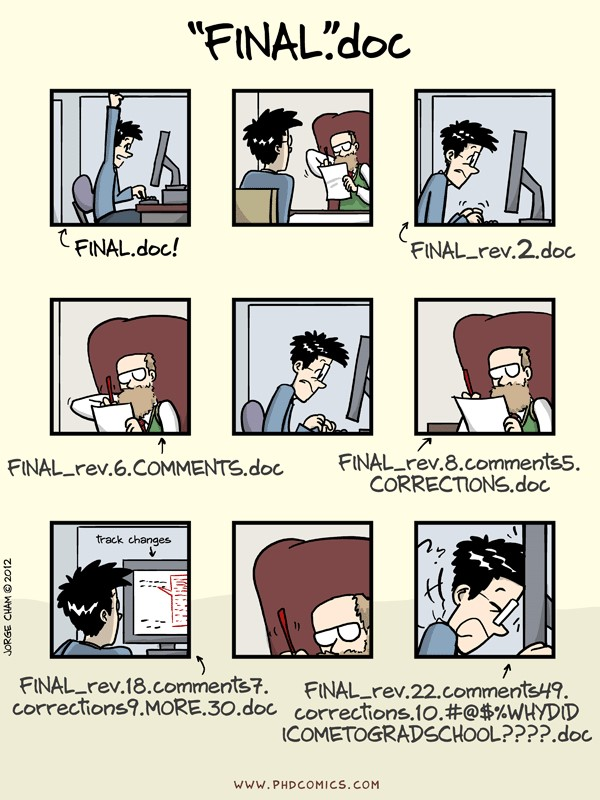
\includegraphics{final.jpg}
\caption{final}
\end{figure}

We'll be talking about the challenge of version control throughout this text - and I am hoping that my own habits in file management can improve as we move forward together.

\hypertarget{discussion-who-deserves-a-good-grade}{%
\section{discussion: who deserves a good grade?}\label{discussion-who-deserves-a-good-grade}}

In an introductory class in data science, students invariably come to class with different backgrounds. Should this be taken into account in assigning grades? That is, would it be possible (and desirable) to assign grades in a class based not just on what students know at the end of the term, but also on how much they have learned?

A formal, statistical approach to this could use regression analysis. That is, one could predict final exam scores from pretest scores, and use the residuals - the extent to which students did better or worse than expected - as a contributor to final exam grades. Interestingly, there would be an unusual incentive for students on this `pretest' to do, seemingly perversely, as poorly as possible. How could this be addressed?

Another problem with this approach is that there may be `ceiling effects' - students who are the strongest coming in to the class can't improve as much as those who have more room to grow. Again, how might this be addressed?

\hypertarget{an-introduction-to-r}{%
\chapter{an introduction to R}\label{an-introduction-to-r}}

R is a system for \textbf{Reproducible research}, and reproducibility is essential \citep{gandrud2016reproducible}.

\begin{quote}
Research is often presented in very selective containers: slideshows, journal articles, books, or maybe even websites\ldots{} these documents are not the research {[}rather{]} these documents are the ``advertising''. The research is the ``full software environment, code, and data that produced the results'' {[}Buckheit and Donoho, 1995, Donoho, 2010, 385{]}. When we separate the research from its advertisement we are making it difficult for others to verify the findings by reproducing them.
\end{quote}

R markdown documents (like Jupyter notebooks in the Python world) facilitate reproducible research, as they include comments or explanations, code, links to data, and results.

\hypertarget{some-other-things-that-r-stands-for}{%
\section{some other things that R stands for}\label{some-other-things-that-r-stands-for}}

Historically, R grew out of S which could stand for Statistics. But what does R stand for?

R is a system for \emph{Representing data} in cool, insight-facilitating ways. R is \emph{Really popular}, and really growing. Learning R will make you a more attractive candidate for many graduate programs as well as jobs in the private sector.

R might stand for \emph{Relatively high level.} Programming languages can be described along a continuum from high to low level, the former (like R) are more accessible to humans, the latter (like assembly language) more accessible to machines. Python, Java, and C++ are all more towards the middle of this continuum.

R stands, in part, for \emph{Resources.} Because R is popular, there are many resources, including, for example -

\begin{itemize}
\tightlist
\item
  Online resources include the simple (and less simple) lessons of \href{http://swirlstats.com/}{SwirlR}, which offers the possibility of ``learning R in R,'' as well as \href{https://www.datacamp.com/home}{DataCamp}, the \href{https://www.coursera.org/specializations/jhu-data-science}{Data Science Certificate Program at Johns Hopkins,} and other MOOCs.\\
\item
  Books include \citet{peng2015r} - which includes not only videos of his lectures in the program at Hopkins, but also a brief list of still more resources - and \citet{wickham2016r}.
\item
  You'll also learn (more directly) from people, including your classmates, as well as the broader community of people around the world. There are hundreds if not thousands of people, young and old, who are on the road with you. I am as well, just a step or two (hopefully) ahead.
\end{itemize}

R does not stand for `\href{https://www.urbandictionary.com/define.php?term=ARGH}{argh},' although you may proclaim this in frustration (`arggh, why can't I get this to work?) or, perhaps, in satisfaction ('arggh, matey, that be a clever way of doing this'). But R does stand for \textbf{\emph{Rewarding}}. A language is a way of thinking about the world, and this is true for computer languages as well. You'll be challenged by its complexity, its idiosyncracy, its alien logic. But you will succeed, and you will find that you can do things that you did not believe possible.

\hypertarget{a-few-characteristics-of-r}{%
\section{a few characteristics of R}\label{a-few-characteristics-of-r}}

R includes the base plus thousands of \textbf{packages}. These packages are customized add-ons which simplify certain tasks, such as text analysis. But there are, at this writing, \href{https://cran.r-project.org/web/views/NaturalLanguageProcessing.html}{over 50 different packages for text analysis} - so where do you begin? One recent answer, and where we will start, is the curated list of packages which jointly comprise the tidyverse \citep{wickham2016r}.

\begin{quote}
A few years ago, \citet{peng2015r} speculated that ``it would be straightforward to build an R package for ordering pizza.'' Does one exist now?
\end{quote}

R is an \textbf{object-oriented} language - one conceptually organized around objects and data rather than actions and logic. In R, at the atomic level, objects include \emph{characters, real numbers, integers, complex numbers, and logical.} These atoms are combined into vectors, which generally include objects of the same type \citep[one kind of object, `lists,' is an exception to this;][]{peng2015r}. Vectors can be further combined into \textbf{data frames}, which are two-dimensional tables or arrays. A \textbf{tibble} is a particular type of data frame which is, in some ways, handier to work with than other data frames. We'll be working extensively with data frames in general, and tibbles in particular, as we move forward.

Objects have attributes. Attributes of R include such things as name, dimensions (for vectors and arrays), class (that's the atomic thing), length, etc.

Real world data sets are messy, and frequently have \textbf{missing values.} In R, missing values may be characterized by NA (not available) or NaN (not a number, implying an undefined or impossible value).

\textbf{R Studio,} the environment we will use to write, test, and run R code, is a commercial enterprise whose business model, judged from afar, is an important one in the world of technology. Most of what R Studio offers is free (97\% according to Garrett Grolemund in the video below). The commercial product they offer makes sense for a relative few, but it is sufficiently lucrative to fund the enterprise. The free product helps to drive the popularity of R studio; this widespread use, in turn, makes it increasingly essential for businesses to use. This mixed free/premium, or `freemium,' model characterizes Slack as well, but while \href{https://www.statista.com/statistics/652779/worldwide-slack-users-total-vs-paid/}{the ratio of free to paid users of Slack is on the order of 3:1}, for R it is, I am guessing, an order of magnitude higher than this.

\hypertarget{finding-help}{%
\section{finding help}\label{finding-help}}

\textbf{one does not simply `learn R.'} Unlike, say, learning to ride a bicycle, fry an egg, or drive a car with a manual transmission, learning R is not a discrete accomplishment that one can be said to have mastered and from which one then moves on. Rather, R is an evolving, open system of applications and tools which is so vast that there is always more that one can achieve, new lessons that one can learn.

So all of us will need help.

For us, the key ideas in ``looking for help'' will include not just the tools on the R Studio IDE, but also (a) using google searches wisely, and (b) reaching out to your classmates on Slack.

There is an etiquette for help-seeking here as in the real world. Your search for help should begin by making sure that others will encounter the same result, then by stripping the problem down to its essence. Once you have reduced the problem to this \emph{minimal, reproducible} essence, you will often be able to spot the problem yourself - and, if not, you will make it easier for others to help you. There is an R package (reprex) which will likely facilitate this, but I haven't tried it yet. \href{https://www.tidyverse.org/help/}{Here} is a good introduction.

Finally, to get a sense of some of the ways you can get help in R studio (and to see how a master uses the R Studio interface), consider this video:

\href{https://www.rstudio.com/resources/webinars/rstudio-essentials-webinar-series-part-1/?wvideo=k8kz4e0p2v}{\includegraphics{https://embedwistia-a.akamaihd.net/deliveries/85f90f89c20cf329c8e6091508fe44c045e70167.jpg?image_play_button_size=2x\&image_crop_resized=960x585\&image_play_button=1\&image_play_button_color=4287c7e0}}

\hypertarget{discussion-is-open-source-software-secure}{%
\section{discussion: is open-source software secure?}\label{discussion-is-open-source-software-secure}}

Perhaps the most important feature of R is that it is open-source software. This is important not just because it saves you money, but because contributing to the world of R is an act of digital democracy. In using and contributing to the world of R we open up knowledge to others who may lack our privileges. R, like Android or Wikipedia, is a tool for all of us, maintained and continually improved upon by the crowd.

But is open-source software safe? More generally, in a data-dependent world, who should be the guardians of the code that connects us?

\textbf{Securing the Internet of Vehicles}. To consider just one example, the computer systems in modern cars typically run millions of lines of code. As cars become increasingly autonomous, this complexity will only increase. (Incidentally, the Society of Automotive Engineers, or SAE, describes 6 levels of `auto autonomy.' At this writing, the most sophisticated systems available to consumers, such as Tesla Autopilot, are at level 2. What lies ahead are cars which are self-driving on carefully selected, geo-fenced roads, and ultimately cars ``\href{https://www.caranddriver.com/features/a15079828/autonomous-self-driving-car-levels-car-levels/}{which can operate on any road\ldots{} a human driver could negotiate}''). Our roads and highways will become an Internet of Vehicles (IOV), which will include not just connections between cars and an intelligent \emph{cloud} `above us' but also direct links between a distributed system of intelligent cars, stoplights, and road sensors in a \emph{fog} `around us' \citep{bonomi2012fog}. \textbf{Fog computing} and the IOV will reduce travel times and increase both fuel efficiency and automotive safety.

Obviously, there are \textbf{cybersecurity} concerns. While the prospects for \href{https://www.youtube.com/watch?v=OvewYslou9g}{a chaotic, choreographed hack of hundreds of vehicles on the streets of Manhattan}, such as that in the 2017 movie ``The Fate of the Furious'', are remote at best (or worst), there have been examples of ``white-hat hackers'' who have successfully infiltrated (and thereby helped secure) car information systems.

As the IOV develops, there will be vulnerabilities to privacy as well as safety, and the security of the system will be paramount. Different car manufacturers are taking different approaches to developing secure information systems, with many using a closed or proprietary approach. But the scope of the problem is so large that there is a movement towards pooling resources and encouraging collaboration among industry partners, academics, and citizen scientists in the development of an open-source autonomous driving platform, such as \href{http://apollo.auto/}{Apollo}. Perhaps counterintuitively, there may be significant security advantages to using source code that is open to all \citep{clarke2009open, fitzgerald2016open}.

\hypertarget{hello-world}{%
\chapter{hello world}\label{hello-world}}

It's time to start moving ahead with R. You can expect a few moments where you feel like you are drawing an owl (origin unknown), but persist!

\begin{figure}
\centering
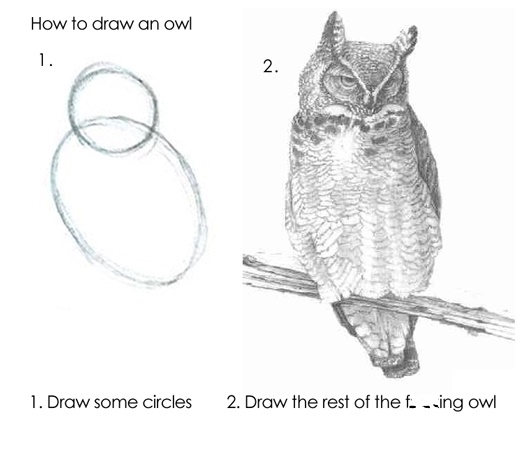
\includegraphics{InkedrCr9A_LI.jpg}
\caption{InkedrCr9A\_LI}
\end{figure}

\hypertarget{wickham-and-r-for-data-science}{%
\section{Wickham and R for Data Science}\label{wickham-and-r-for-data-science}}

The first chapter of the Wickham text provides a framework for his approach and a brief introduction to the \emph{tidyverse.}

After you have read this, please \textbf{spend at least 90 mins} exploring at least one of the following. Be prepared to discuss your progress next class (you will be asked which source(s) you used, what you struggled with, and whether you would recommend it to your classmates:

\hypertarget{additional-sources}{%
\section{Additional sources:}\label{additional-sources}}

\hypertarget{carmichael}{%
\subsection{Carmichael}\label{carmichael}}

Iain Carmichael prepared the following for his Intro to Data Science course at UNC-Chapel Hill. I think it is a great place to start: \url{https://idc9.github.io/stor390/notes/getting_started/getting_started.html}

\hypertarget{datacamp}{%
\subsection{DataCamp}\label{datacamp}}

Many folks swear by (and others, I presume, at) DataCamp, which kind of gamifies learning software. As a student in this class, you have access to all of their stuff\ldots{} free. You can even do lessons on your phone.

\hypertarget{swirl-swirlstats}{%
\subsection{Swirl (Swirlstats)}\label{swirl-swirlstats}}

I, like thousands of others, learned R in the process of completing the Johns Hopkins \href{https://jhudatascience.org/courses.html}{Data Science Specialization} offered through Coursera. The sequence can be challenging, but their introduction to R used an accessible, interactive R package called \emph{Swirl.} You can read about swirl (``learn R in R'') at \url{https://swirlstats.com/}.

\textbf{Using Swirl.} After loading R (and opening R studio), you will get to the Swirl lessons with the following steps:

\begin{enumerate}
\def\labelenumi{\arabic{enumi})}
\tightlist
\item
  Install the Swirl package on your computer (you only need to do this once). Type the following into your console window in R studio (typically left hand side of your screen or lower left)
\end{enumerate}

\begin{quote}
install.packages(``swirl'')
\end{quote}

\begin{enumerate}
\def\labelenumi{\arabic{enumi})}
\setcounter{enumi}{1}
\tightlist
\item
  Then load the package into your workspace (you'll need to do this at the beginning of every session you use Swirl)
\end{enumerate}

\begin{quote}
library (swirl)
\end{quote}

\begin{enumerate}
\def\labelenumi{\arabic{enumi})}
\setcounter{enumi}{1}
\tightlist
\item
  Then run it!
\end{enumerate}

\begin{quote}
swirl ()
\end{quote}

Swirl will ask a few questions then give you the option of choosing one of several courses. You'll choose the R Programming option, which leads to 15 separate lessons.

At the end of each lesson, you'll be asked

\begin{quote}
\emph{Would you like to receive credit for completing this course on Coursera.org?}
\end{quote}

Answer no\ldots{} then do another lesson.

\hypertarget{peng-text-and-videos}{%
\subsection{Peng text and videos}\label{peng-text-and-videos}}

Finally, consider the text and videos from the Coursera R class. Most of the material from that class can be found in \citet{peng2015r}. A slightly updated version of the text can be found at \url{https://bookdown.org/rdpeng/rprogdatascience/}, and the videos in the series may be found by clicking on the following:

\href{https://youtu.be/wy0h1f5awRI}{\includegraphics{https://img.youtube.com/vi/wy0h1f5awRI/0.jpg}}.

\hypertarget{part-part-ii-towards-data-literacy}{%
\part{Part II Towards data literacy}\label{part-part-ii-towards-data-literacy}}

\hypertarget{principles-of-data-visualization}{%
\chapter{Principles of data visualization}\label{principles-of-data-visualization}}

\hypertarget{opening-thoughts}{%
\section{Opening thoughts}\label{opening-thoughts}}

Graphs aren't just to inform, but to make you reflect.

We are concerned not just with the design of graphs, but with our role in society as leaders, as arbiters of facts, as educators. We want to foster data literacy.

How do people understand graphs? (NY Times series for schools).

How can you use graphs to tell people the truth in a way that they understand?

When you see a graph, what do you notice, what do you wonder, and what is the story? Is ``story telling'' what visualizations should be about?

A graph might begin with perception and understanding (the consumer), with knowledge and design values (the producer), but it also reflects the truth of the data. How much is each?

\hypertarget{some-early-graphs}{%
\section{Some early graphs}\label{some-early-graphs}}

Visual displays of information reach back to prehistoric times; modern graphs date back, arguably, to Playfair's 1786 \emph{Political Atlas} - in which

\emph{``\ldots{} spatial dimensions were used to represent nonspatial, quantitative, idiographic, empirical data. Although it now seems natural to represent, for example, rising and falling imports over time as a rising and falling line, it does not seem to have been done before that time and was quite an accomplishment. Notably, in addition to the statistical line chart, Playfair at one fell swoop single-handedly invented most of the remaining forms of the statistical graphic repertoire used today-the bar chart and histogram, the surface chart, and the circle diagram or''pie chart."}

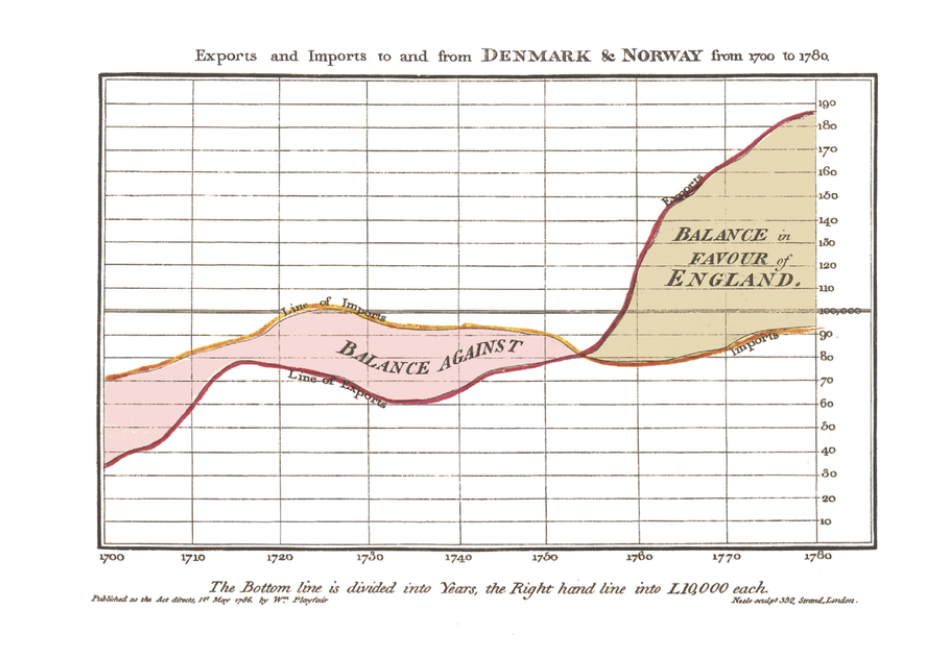
\includegraphics{playfair1786.PNG}\href{https://robots.thoughtbot.com/analyzing-minards-visualization-of-napoleons-1812-march}{source}

\begin{center}\rule{0.5\linewidth}{\linethickness}\end{center}

\begin{enumerate}
\def\labelenumi{\arabic{enumi})}
\setcounter{enumi}{1}
\tightlist
\item
  The most important early graph is that of Minard. Here's some background:
\end{enumerate}

"\emph{Czar Alexander of Russia sees that Napoleon was becoming too powerful, so he refuses to participate in this embargo. Angry at Czar Alexander's decision, Napoleon gathers a massive army of over 400,000 to attack Russia in June of 1812. While Russia's troops are not as numerous as France's, Russia has a plan. Russian troops keep retreating as Napoleon's troops move forward, burning everything they pass, ensuring that the French forces could not take anything from their environment. Eventually the French army follows the Russian army all the way to Moscow during October, suffering major losses from lack of food. By the time Napoleon gets to Moscow, he knows he has to retreat. As winter settles into Europe and the temperature drops, Napoleon's troops suffer even more losses, returning to France from lack of food, disease, and weather conditions."}

In class, we listened to the 1812 Overture while discussing this.

(The battle of Borodino, immortalized in Tolstoy's War and Peace, occurs just before Moscow; the French army loses about 30000 men. Five cannon shots in the overture mark this. And when Napoleon gets to Moscow, he finds that the Russians had razed it before hand, so that there was nothing there for them. Eleven more cannon here.)

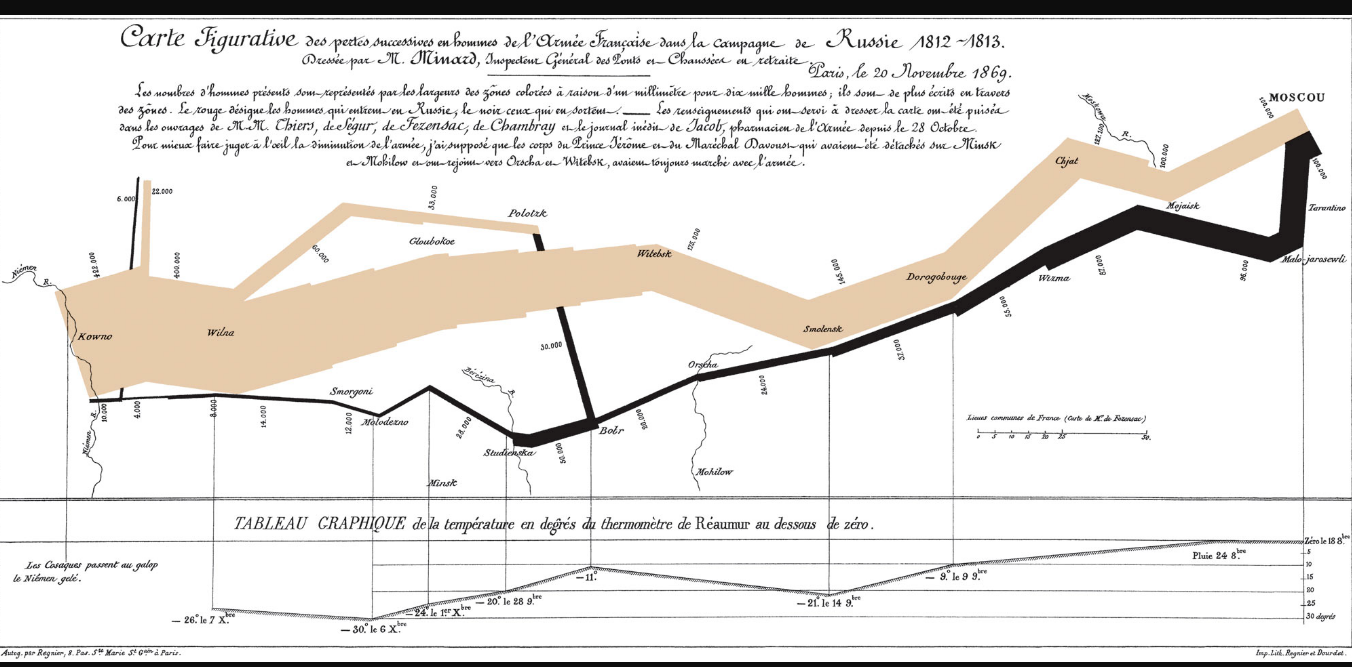
\includegraphics{minard1812.PNG}\href{https://datavizblog.com/2013/05/30/dataviz-history-charles-minards-flow-map-of-napoleons-russian-campaign-of-1812-polotsk-smolensk-and-on-to-borodino/}{source}

\begin{center}\rule{0.5\linewidth}{\linethickness}\end{center}

\hypertarget{tukeys-contributions}{%
\section{Tukey's contributions}\label{tukeys-contributions}}

Tukey and Exploratory Data Analysis (EDA). Begins with Tukey 1962 ``Future of Data Analysis,'' continues with his ultimate publication of EDA in 1977.

Tukey decries tallies (prone to error), and shows \textbf{stem and leaf displays}, then box plots. He argues for transforming data to linearity to uncover meaningful relationships, then to examine residuals to look more closely.

\hypertarget{approaches-to-graphs}{%
\section{Approaches to graphs}\label{approaches-to-graphs}}

A graph might begin with perception and understanding (the consumer), with knowledge and design values (the producer), but it also reflects the truth of the data. How much is each?

In thinking about how to design graphs, we can begin with abstract theory, with principles of design informed by our understanding of perception, or with empirical analyses of understanding and memory.

\hypertarget{tufte-first-principles}{%
\section{Tufte: First principles}\label{tufte-first-principles}}

\citet{tufte2001visual} describes \textbf{Graphical Excellence}. Graphs should, among other things, ``Induce the viewer to think about the substance, rather than about methodology, graphic design, the technology of graphic productions, or something else.'' Graphs should ``Present many numbers in a small space, make large data sets coherent, and encourage the eye to compare different pieces of data.'' Graphs should ``serve a reasonably clear purpose: description, exploration, tabulation, or decoration {[}and{]} be closely integrated with the statistical and verbal descriptions of a data set.''"

Tufte concludes with the following Principles of Graphical Excellence, which I quote verbatim:
\textbf{\emph{Graphical excellence is the well-designed presentation of interesting data---a}}
\textbf{\emph{matter of substance, of statistics, and of design.}}
\textbf{\emph{Graphical excellence consists of complex ideas communicated with clarity,}}
\textbf{\emph{precision and efficiency.}}
\textbf{\emph{Graphical excellence is that which gives to the viewer the greatest number of}}
\textbf{\emph{ideas in the shortest time with the least ink in the smallest space.}}
\textbf{\emph{Graphical excellence is nearly always multivariate.}}
\textbf{\emph{And graphical excellence requires telling the truth.}}

\begin{center}\rule{0.5\linewidth}{\linethickness}\end{center}

\hypertarget{an-illustration-of-the-cost-of-bad-graphs-the-challenger-disaster}{%
\subsection{An illustration of the cost of bad graphs: The Challenger disaster}\label{an-illustration-of-the-cost-of-bad-graphs-the-challenger-disaster}}

\begin{figure}
\centering
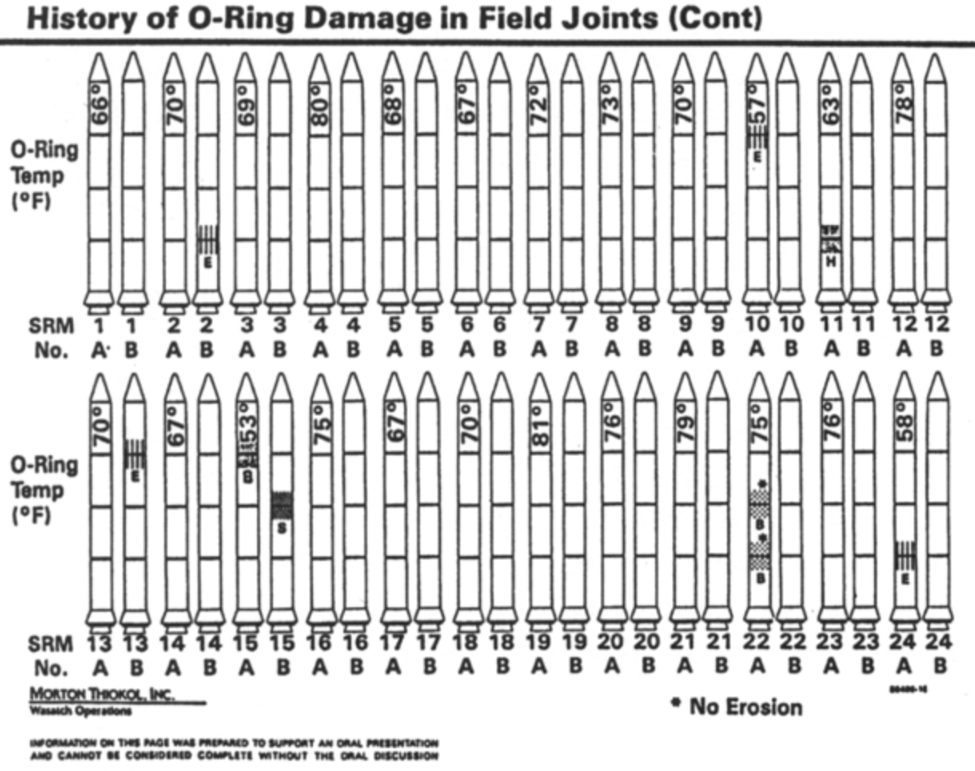
\includegraphics{mortonthiokolChallenger.PNG}
\caption{mortonthiokolChallenger}
\end{figure}

\begin{figure}
\centering
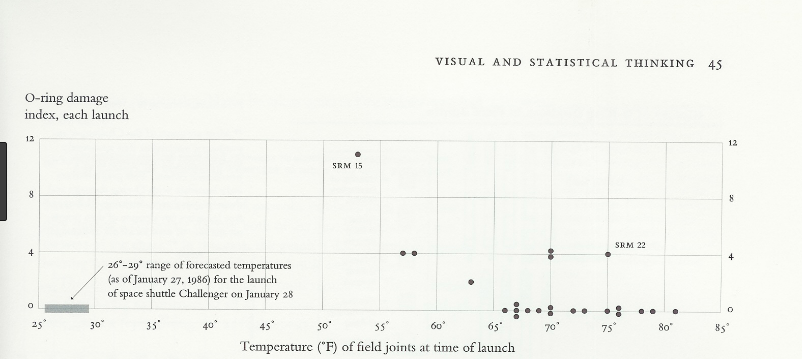
\includegraphics{tufteChallenger.PNG}
\caption{tufteChallenger}
\end{figure}

\hypertarget{should-graphs-begin-with-psychological-theory}{%
\subsection{Should graphs begin with psychological theory?}\label{should-graphs-begin-with-psychological-theory}}

\citet{wainer1981graphical} used Chernoff's faces to represent multivariate data. Grounded in a psychological premise. Did they succeed? Why or why not?

\begin{figure}
\centering
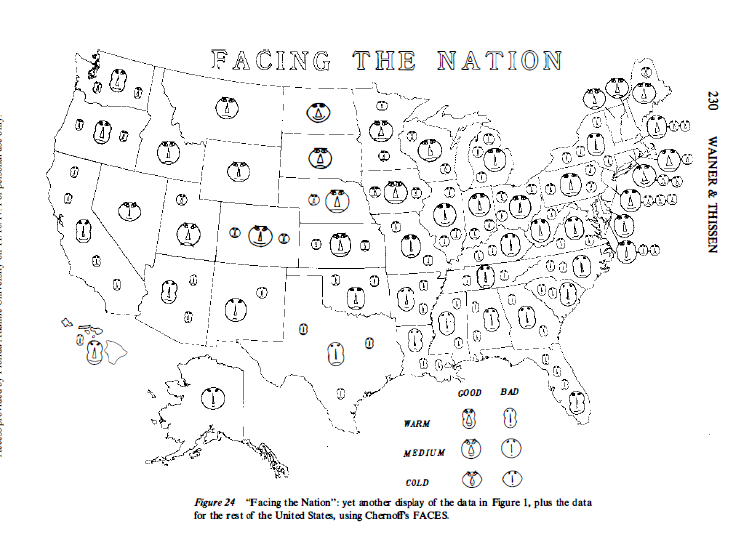
\includegraphics{Chernoff.PNG}
\caption{Chernoff}
\end{figure}

Population - the (log) number of faces/state

Literacy rate - size of the eyes (bigger = higher).

\% HS graduates - slant of the eyes (the more slanted = higher).

Life expectancy - the length of the mouth (the longer = longer).

Homicide rate - the width of the nose (the wider the nose the lower).

Income - the curvature of the mouth (the bigger the smile the higher the income).

Temperature - the shape of the face (peanut= warmer, football= colder)

Longitude and latitude - The X and Y position of the face on the coordinate axes of the paper represent the position of the state

\hypertarget{the-power-of-animation}{%
\subsection{The power of animation}\label{the-power-of-animation}}

This section concludes with two brief (\textless{} 5 minutes) animated data displays, each powerful in its own way, and each giving the viewer an appreciation of an important social phenomenon.

The first is from the late Hans Rosling, and summarizes a chunk of the Gapminder data. There is a Gapminder package in R if you would like to explore the data further, and perhaps become the next Rosling:

\href{https://youtu.be/jbkSRLYSojo}{\includegraphics{https://img.youtube.com/vi/jbkSRLYSojo/0.jpg}}.

The second is from Kim Rees and her ex-colleagues at \href{https://periscopic.com/}{Periscopic} (Rees is now at CapitalOne). For me, it's an important graphic because it shows an approach to overcoming what has been called ``psychic numbing'' - we are sensitive to the individual case, but lose our perspective when faced with large-scale tragedies, so that effectively the \citep{slovic2013psychic}

\href{https://youtu.be/8R8UOjMy-5k}{\includegraphics{https://img.youtube.com/vi/8R8UOjMy-5k/0.jpg}}.

\hypertarget{further-reading-and-resources}{%
\section{Further reading and resources}\label{further-reading-and-resources}}

This is only the beginning of a discussion of data visualizations. \citet{healy2018viz} presents a more expanded discussion of this treatment. He addresses the limitations of infographics, in which the design purveys style over substance (this is what we may do in designing presentations as well), and includes a rationale for a grammar of graphics, as instantiated in the ggplot package in R that we will be working with beginning next week \citep{wickham2016r}. \citet{cleveland1985graphical} examines graphs from a more rigorous psychological and empirical viewpoint. The \href{http://datastori.es/}{Data Stories podcasts} are often excellent, despite the challenge of an auditory medium for visual display. And your classmates and instructors have things to say as well.

\hypertarget{references}{%
\chapter{references}\label{references}}

\bibliography{../9Bibliography/dataSciRefs.bib}


\end{document}
